\section{Generating bill based Policy Networks}\label{sec:implementation}

In this study we propose to use bills approved by a Parliament as the element linking political actors. To generate a PN, we take as input news articles and Parliamentary data and automatically model topics based on the contents of the bills, extract relevant politicians that participated in the drafting of the bill, find articles related to each of these topics, perform entity recognition and normalization and compute similarity measures between relevant entities to produce \emph{Entity-entity graphs}. Figure \ref{fig:pipeline_bill} shows the pipeline of the whole process, from the obtention of the data to the production of the desired graphs. In this chapter we describe how we carry out each of these tasks. \\

\begin{figure}[h!]
    \centering
    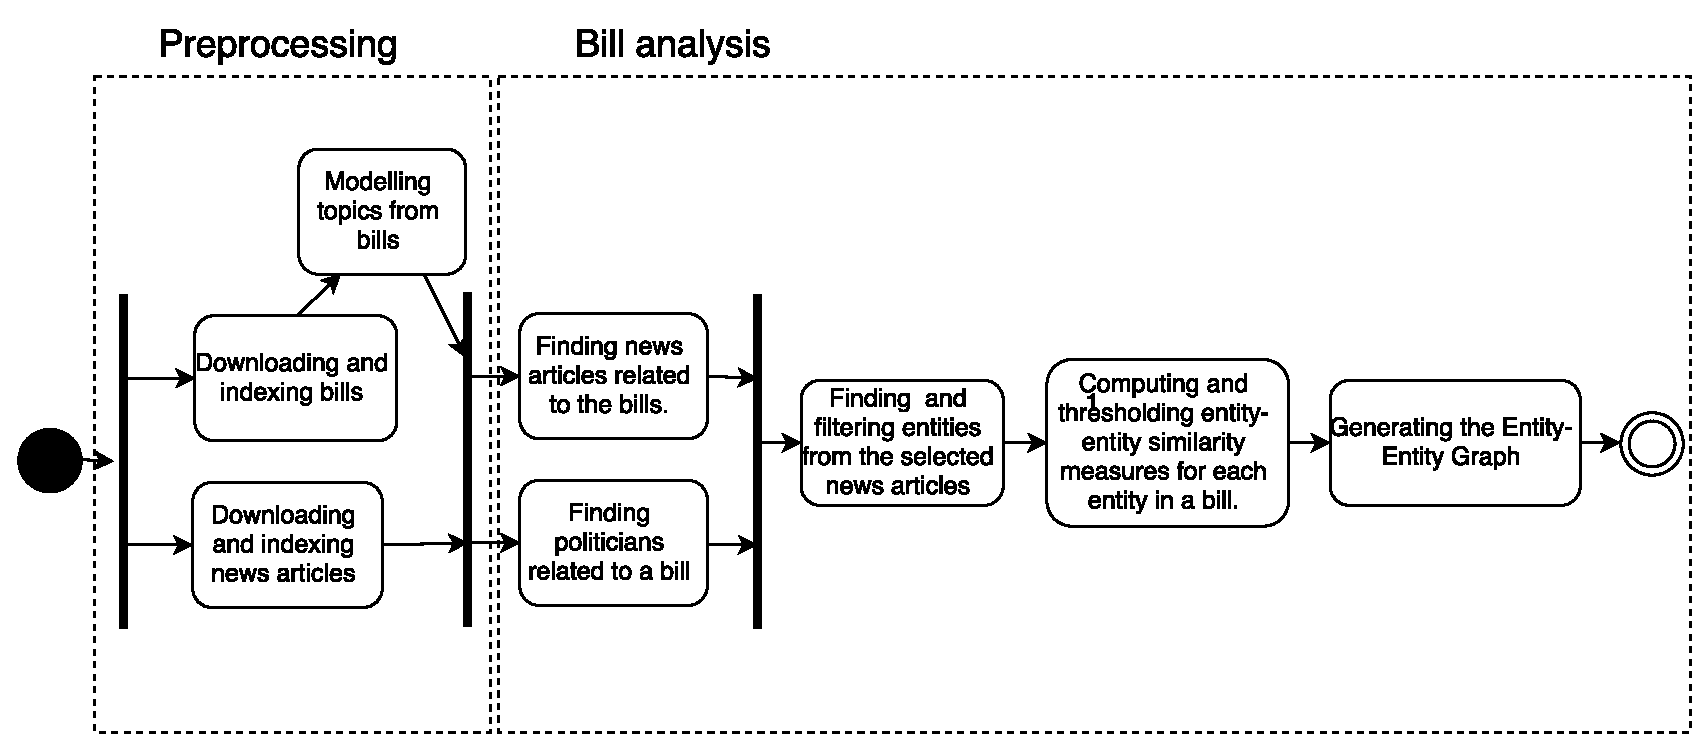
\includegraphics[width=1\textwidth]{figs/Analyze_bill}
    \caption{The pipeline of our bill analysis.}
    \label{fig:pipeline_bill}
\end{figure}

\subsection{Preprocessing: getting the data ready for analysis} \label{subsec:preprocessing}

The first step consists of obtaining and preprocessing the news articles and bills so that they can be analyzed efficently. To do this, we developed scrappers to automatically visit the websites of the main newspapers of Catalonia and download all the news articles of the last ten years. This requires a different approach for each newspaper, particularly to determine how to get to every news article from their home page and the Xpath necessary to get the contents of the news articles without noise. We also made a scrapper to download all the bills that have been approved by the Catalan Parliament. \\

In Catalonia many newspapers publish their articles in Catalan or Spanish, or in some cases both. For this study, we chose to work only with news articles written in Spanish. The reason is that there are better Entity Recognition tools for Spanish. To automatically classify the articles by language, we use the number of stopwords in Spanish and Catalan of each article. After doing this process we obtained a total of 758276 articles in Spanish. \\ 

Once we have downloaded the news articles, we index them using ElasticSearch\footnote{https://www.elastic.co/}, a distributed search engine based on Apache Lucene. ElasticSearch uses inverted indices to fastly query documents. Based on the types of queries that we do, we make two indices treating news article and individual paragraphs as documents.

\subsubsection{Modelling topics from bills}\label{subsec:extract_topic}

We model each bill as a topic by extracting a list of weighted keywords. This allows us to find news articles that are related to each bill. To find keywords, we consider n-grams of size \emph{1,2,3} and compute the TF-IDF score of these n-grams with respect to the set of all bills approved by the Parliament. TF-IDF is a measure of relevance of a keyword in a specific document which takes into account its frequency inside the document and accross the whole corpus of documents. Formally, it is defined as:

$$ tf-idf(keyword,document,corpus) = tf(keyword,document) * idf(keyword,corpus)$$

Where tf is usually the number of times that the keyword occurs in the document and idf is the \emph{inverse document frequency}, a term which aims to penalize words that are used in many documents, and is defined as:

$$ idf(keyword,corpus) = log(\frac{|corpus|}{|\{d \in corpus | keyword \in d\}|})$$

For computing the TF-IDF of a keyword, we consider each bill as a document. \\

To enhance the quality of the keyword extraction we could also consider the transcripts of the debates of each bill. By doing this we could discover words and phrases that describe the contents of the bills in an informal, non-legislative way which is possibly more similar to the jargon used by newspapers. This is however a minor improvement and is left for future work. \\

After extracting keywords, we rank them and keep the top 1000 keywords. We keep the TF-IDF score of the keywords as a weight. 

\subsection{Analyzing a bill} \label{subsec:bill_analysis}

To analyze a bill, we find relevant politicians and related news articles, detect relevant entities and compute entity-entity similarity measures to generate the desired Social Networks. In this section we describe this process in detail.

\subsubsection{From bills to news articles: modelling topics from bills }\label{subsec:topic}

In order to find entities that are related to the bills, we first find news articles that are related to the bills. To do this, we use the extracted keywords to query the corpus of news articles. To determine the relevance of an article, we consider the vector space model representation of each bill and news article, and compute the cosine similarity between the vectors. \\

To improve the phase of keyword extraction, we use Rocchio's algorithm to discover new keywords from the corpus of news articles. Rocchio's algorithm is widely used in Information Retrieval systems to expand queries defined by users by adding news terms found in the top relevant documents retrieved by an initial search. To determine what a relevant document is there are two alternatives: (i) asking the user for feedback -- an option which is not possible in our application -- and ii) assume that the top documents retrieved by the query are relevant. \\

After defining a set of relevant documents $|R|$ and a set of non-relevant documents, we update the query vector $q$ according to this formula: \\

\begin{eqnarray*}
q_{new} = \alpha* q +  \beta * \frac{1}{|R|} * \sum_{d \in R}{d} + \gamma * \frac{1}{|NR|} * \sum_{d \in NR}{d} \\
\end{eqnarray*}

Where d is a document in the vector space model, $\alpha, \beta, \gamma $ are manually fixed parameters usually satisfying $\alpha > \beta > \gamma = 0$. \\

Once a new query vector is computed, we execute a new query and rank the news articles according to the new query. After doing this, we need to determine the number of articles to use based on the score. To do this, we plot the score of the articles with respect to their ranking and find the best trade-off point according to the following method.

\subsubsection{Finding the best trade-off point between relevance and size}\label{subsec:elbow}

When plotting a relevance as a function of the ranking of an article, we observe that all bills follow a pattern similar to the one in figure \ref{fig:articles-topic-threshold}. That is, the relevance score is very high for the first articles and then drops quickly. We want to use as many relevant articles as possible, avoiding at the same the inclusion of articles that are not related to the bill and that could introduce noise. \\

\begin{figure}[h!]
    \centering
    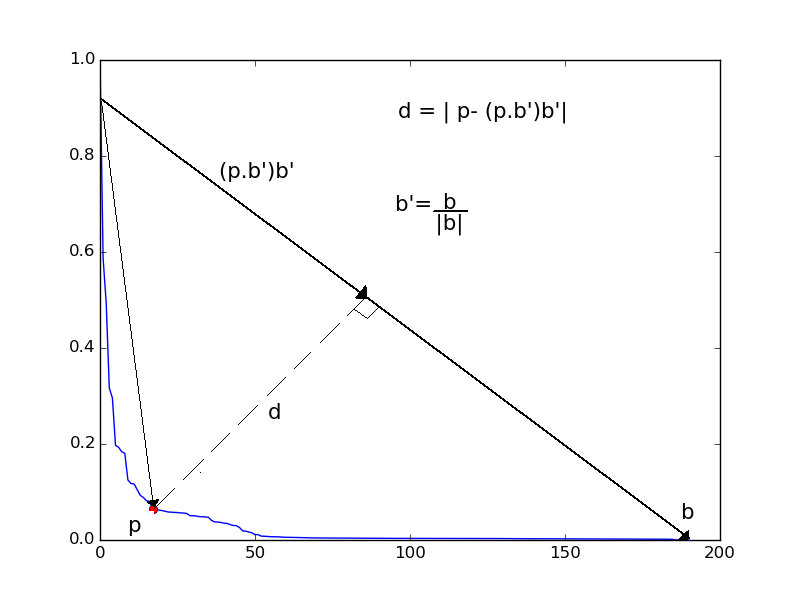
\includegraphics[width=0.7\textwidth]{figs/articles-topic-threshold2}
    \caption{Determining the number of articles to use for a given bill.}
    \label{fig:articles-topic-threshold}
\end{figure}

To solve this, we observe that the plot ressembles an elbow and pick a value a point near the region where the two arms of the elbow meet. One way to do this is by selecting the point $p$ that maximizes $d$ as shown in figure \ref{fig:articles-topic-threshold}. In the figure:

\begin{itemize}
\item $b$ is a vector pointing from the point of highest relevance to the point of lowest relevance.
\item $b'$ is an unitary vector in the direction of $b$
\item $p$ is a vector pointing from the point of highest relevance to each point in the curve.
\item $(p.b')b'$ is the projection of $p$ onto $b$.
\item $|p - (p.b')b'|$ is the distance of every point of the curve to the line going from the point of highest relevance to the point of lowest relevance.
\end{itemize}

The threshold is chosen by determining the point that maximizes d according to the formula:

$$threshold = \underset{p} {\mathrm{argmax}} |p - (p.b')b'|$$


\subsubsection{From news articles to political actors: entity recognition and preprocessing}\label{subsec:getting-entities}

After finding articles related to bills, they are analyzed to find entities that are in turn related to the bills. For this purpose we use MITIE\footnote{https://github.com/mit-nlp/MITIE}, a state of art tool Named Entity Recognition tool created by the MIT. Given a document, MITIE identifies substrings that contain possible named entities and tags them as \emph{Organization, Location, Person} or \emph{Miscellaneous}.\\

Before carrying on the detected entities need to be pre-processed before they can be used. The names found may i) not be correctly delimited (resulting in truncated names or in names that contain excess text) ii) be ambiguous (an entity may have more than one name and a name may refer to more than one entity) and iii) may be noise and not refer to a real entity. \\

Name disambiguation is in itself a complex and interesting research topic which goes beyond the scope of this study. We have however implemented some heuristics we briefly describe below:\\

\begin{enumerate}

\item \textbf{Entity Normalization}: entities are brought to a canonical form to address spelling variations. This involves i) punctuation sign removal; ii) double, leading and trailing whitespaces removal; iii) leading and trailing stop words removal; iv) string camelization (all characters are put in lowercase except for the first letter of every word, which is in uppercase). 

\item \textbf{Mapping organization initials to the whole name}: when an organization name is detected we aim to detect if there are any other names composed by its initials. Specifically, we aim to exploit a widely found pattern: organizations often have the full name followed by the initials inside parenthesis. 

\item \textbf{Mapping partial names with full names}: when person names are detected we classify them into \emph{full names} (containing more than 1 word) and \emph{short names} (containing one word, which is possibly the last or first name of the full name). We then link short names with the nearest, previous full name such that the short name is contained inside the full name.

\item \textbf{Expanding names based on the news corpus}: to address the issue of truncated names (eg `Word Life Fund' may be truncated and processed as `World' and `Life Fund')  we: i) look up every name and its surrounding context in the corpus ii) extract sentences in the top articles and iii) find the longest substring matching these sentences. 
\end{enumerate}

By doing this we find a list of entities for which we have a list of aliases and a list of tag counts. After doing this, we choose for every entity the tag with the highest frequency as the type of the entity. \\

\subsubsection{Extracting the authors and influencers of a bill from Parliamentary data.}\label{political-actors-from-parliamentary-data}

While news articles are an excellent source to determine third party actors which are affected or interested in a bill, there is also a wealth of information to be obtained from open data released by Parliaments. By using the transcripts of their meetings, we can determine who are the authors and the politicians that participated in the drafting of a bill. These politicians might be of great importance and still not show up often in the news articles. \\

In the case of the Catalan Parliament, all the transcripts and procedings of the meetings of the different comissions are available online. The Parliament website also allows to look for the speeches of individual politicians or to look for all the interventions concerning a bill. By interventions we mean speeches, authorships or amendment writing. Given a bill, we label a politician as relevant if they have at least one intervention about that bill. \\

The extraction of relevant politicians could be perfomed automatically by scraping the website of the Parliament or by querying their database. However, due to time constraints this functionality is left for future work. We manually look for each of the bills we analyzed and store the list of relevant politicians in the database. \\

\subsubsection{Selecting relevant actors: filtering noisy entities}

After obtaining a list of entities for each bill, we need to select the entities that are most likely to be related to the bill. Our method for entity selection yields thousands of entities for each of the topics. This makes filtering them necessary for two reasons. \\

First, noise is bound to be present in the list of entities found by our system. This includes entity names that do no correspond to real entities, entities that occur in articles related to the bills but that are not really related to them and entities from articles that are completely unrelated to the bills. As we will see later in section \ref{entity-entity-sim} to compute entity-entity similarity measures it is better to work with a list of entities as less noisy as possible. \\

Second, to produce an entity-entity graph we need to compute similarity measures between each pair entities; the cost of each comparison depends on the method chosen and the number of comparisons to make grows quadratically with the number of entities. \\

To select relevant entities, we first filter out entities that occur less than a given threshold in the whole corpus of news articles. This is useful for removing phrases that are not real entities but that were incorrectly classified as such by the ER tool. Then we compute a gross and inexpensive similarity measure between entities and use it to perform clustering. We do this to find a group of entities that are strongly related among themselves and with the bill. The similarity measure is computed as follows:

\begin{enumerate} 
\item First we generate a binary matrix in which rows correspond to entities and columns correspond to news articles related to the bill that the entities occur in. Each cell contains a one iff the entity occurs in the document; otherwise it contains a zero.   
\item After generating an \emph{Entity-Document} matrix, we perform Latent Semantic Index (LSI) to reduce the number of dimensions. LSI uses Singular Value Decomposition to identify relationships between terms and concepts in a corpus of text. The idea is that terms (in our case entities) that occur in the same context (news articles) tend to have a similar meaning. LSI takes as an input the \emph{Entity-Document} matrix $B$ and transforms it into three matrices: 

\begin{itemize}
\item An $m\times r$ term-concept matrix T, where m is the number of terms and r is the number of concepts.
\item An $r\times r$ singular values matrix S. 
\item An $n\times r$ concept-document matrix, where n is the number of documents.
\end{itemize}

Such that B,T,S and D satisfy the condition:

$$ B \approx TSD^T $$.

By doing LSI we can use the term-concept matrix T to identify that two entities are similar even if they do not co-occur in any documents. The reasoning is that there might be more than one topic (or concept) in the set of retrieved news articles. By automatically identifying possible concepts, we can establish the similarity between two entities based on their relations to the latent concepts as opposed to the stricter requirement of direct document co-occurence.

\item We compute an entity-entity similarity measure by taking the cosine similarity of the entity vectors in the concept space, i.e. the cosine similarity of the rows of the T matrix.

\end{enumerate} 

Computing the similarity measure on the concept space is relatively cheap computationally as it involves computing the dot product between two vectors with few components. We can further reduce the computational cost of selecting relevant actors by using the fact that any entity which is related to the topic must be vaguely related to the politicians that participated in the drafting and discussion of the bill. That is, rather than computing the $N^2$ comparisons involving thousands of entities, we can first compute the similarity of each of the $N$ entities with a list of seed politicians and discard entities which do not have a similarity higher than a certain threshold with at least one of the politicians. We use an $\epsilon = 0.1$ in our system. This is a safe assumption as the seed politicians must be strongly related to the concepts to which the bill is related and are also rows of the B matrix. \\

After computing the similarity measure between all pairs of entities, we perform Hierarchical Aglomerative Clustering (HAC) to identify the set of relevant actors. We define the dissimilarity between two entities as one minus their cosine similarity. More specifically, we perform Unweighted Pair Group Method with Arithmetic Mean (UPGMA), which computes a dendogram that reflects the structure in the dissimilarity matrix. UPGMA uses a bottom-up approach, starting from clusters containing each individuals and progressively merging two clusters at a time until every individual is in the same cluster. At each iteration, the nearest two clusters are combined into a higher-level cluster. UPGMA uses the mean dissimilarity to merge clusters. That is, the dissimilarity between any two clusters A and B is taken to be the average of all dissimilarity between pairs of objects "x" in A and "y" in B. \\

When performing HAC, it is necessary to set a threshold or number of clusters. To select this threshold, we use the silhoutte, a widely usely measure of the quality of a cluster based on the dissimilarities between objects inside a cluster and their dissimilarity with the nearest clusters. Formally, the silhoutte of an observation (in our case an entity) is defined in \cite{rousseeuw1987silhouettes} as:

$$s(i) = \frac{b(i)-a(i)}{max(a(i),b(i))}$$\\

where $a(i)$ is the average dissimilarity of the entity $i$ with the rest of the entities in its cluster and $b(i)$ is the lowest average dissimilarity  of $i$ with any cluster of which it is not a member. \\

It can be shown that $ -1 < s(i) <1 $. Particularly, in order to have a silhoutte close to 1, we need $a(i)>b(i)$, which means that entity $i$ is significantly closer to the members of its cluster than to the members of the nearest cluster. A high value of the silhoutte thus indicates a better cluster quality. We can compute the silhoutte of a cluster by taking the average of all its entities.\\

By taking into account the seed politicians we can choose the best cluster that groups entities related to the bill. We do this by choosing the cluster that i) contains all the seed politicians,  and ii) has the highest average silhoutte.  Because the silhoutte can have several local minima and be unstable  we also request the cluster containing the seed politicians to have a minimum size (we use a minimum size of $100$).\\

After performing this step we are able to reduce the number of entities to analyze from thousands to hundreds. This makes the fine-grained similarity measures we use in section \ref{entity-entity-sim} faster to compute and more accurate.

\subsubsection{From a list of relevant actors to a Policy Networks: computing and thresholding similarity measures}\label{entity-entity-sim}

Once we have produced a list of relevant political actors, we need to compute and threshold a similarity measure to produce a Social Network. Thresholding this similarity measure is an optional step; depending on the type of analysis we wish to perform we could consider all the possible relationships between all the pairs of entities and keep the similarity measure as a weight. We present a method for thresholding this measure however, as it leads to a richer visualization and the analysis and applications that we present in this thesis better with sparse, unweighted graphs.\\

As we previously said in section \ref{subsec:objectives}, we are interested in generating \emph{Entity-Entity graph} capturing relationships between entities that given the context of a bill, share similar roles or positions. The challenge of this procedure is thus being able to determine which are the relevant relationships between the entities without i) producing very dense graphs (high number of edges) and ii) missing important relationships. \\

As we saw in chapter \ref{sec:related-works}, the state of the art in SN generation uses co-occurence and topic modelling to compute the similarity between two entities. In this study we use a text-based similarity measure similar to the one used by the authors of \cite{policy-networks}. Its computation consists of the following steps:

\begin{enumerate}
\item For every entity, look for every article that mentions it which is related to the bill. We consider that an article is related to the bill if it is selected after applying the elbow criterion specified in section \ref{subsec:elbow}. 
\item For every article the entity is mentioned in, look for every paragraph that mentions the whole name of the entity or any of its aliases.
\item For every paragraph that mentions the entity, generate $1,2,3$ grams with the contents of the paragraph. Then use these N-grams to generate a vector space representation of the entity capturing the contexts it is talked about. We use TF-IDF to generate these vectors, using sublinear tf scaling in which the TF component is calculated as follows:

$$tf = 1+ log(frequency)$$ 

This version of TF-IDF is widely used when the weight of a keyword should not be linearly dependent on its number of occurrences. For instance, a keyword occurring 30 times should not be 30 times more important than a keyword occurring only once. This is useful in our context as we are comparing N-grams of different sizes and using normal TF-IDF could give much more weight to N-grams of size one over N-grams of size two or three, as n-grams of size one are more likely to have a higher frequency. The N-grams of size three could however be more useful to describe the entities. Also note that this version gives a higher weight to the IDF component of the formula, as $1+log(x)>x$ for $x>1$. This means that we also give a higher weight to rare terms in comparison with the typical TF-IDF formula.
\item The similarity between two entities is finally computed by taking the cosine similarity of the vectors representing each entity.  
\end{enumerate}

This similarity measure has several of the advantages of the different approaches we studied in the literature. Specifically, it takes into account:

\begin{itemize}
\item Entity co-occurence in a context: if two entities are mentioned together, they will be represented in their corresponding vectors as N-grams. Furthermore by using TF-IDF the co-occurence is weighted according to its frequency -- if two entities co-occur often their corresponding components will be high -- and the frequency of each entity accross all the documents -- if an entity is often referred to, then the IDF will penalize its weight --.
\item The semantic role of the entity with respect to the topic, as captured by the words that are used to talk about that entity and the bill.
\end{itemize}

Note that by using only documents that specifically talk about a bill, we are able to produce fine-grained similarity measures. If we tried to determine the similarity based on the whole set of documents, the relationships between politicians and actors that are rarely talked about could be missed. The N-grams that describe each entity are computed  and weighted taking into account only news articles that talk about the bill. \\

The last step before computing the PN consists of thresholding the similarity measure to discard relationships between entities that have a low weight. Rather than using a global threshold for all the relationships, we fix a threshold for each entity taking into account its similarities. For each entity $e$ we:

\begin{enumerate}
\item Rank the rest of the entities with respect to their similarity to $e$.
\item Plot the similarity measure of every entity with respect to $e$ as a function of the ranking.
\item Find an elbow according to the method defined in \ref{subsec:elbow}. This elbow captures the most relevant entities for $e$, i.e., it detects the point after which all entities have a low similarity. This decision was made empirically after studying the similarity-ranking plots of several entities for different bills; most of the plots follow the shape of figure \ref{fig:articles-topic-threshold}, meaning that the elbow is an useful technique for filtering relevant entities.
\end{enumerate}


After computing a set of relevant entities for each entity, we decide that two entities $e1$ and $e2$ are related iff they are included in the set of relevant entities of the other entity. That is, $e1$ must be contained in the list of relevant entities of $e2$ and viceversa. This requirement implies that two entities must be \emph{strongly} related to be added to our final graph. Note that an interesting variant consists of considering instead directed graphs in which we draw an edge from a node $e1$ to a node $e2$ if $e2$ is a relevant entity for $e1$ or if $e1$ is a relevant entity for $e2$. Studying this alternative is left for future work. \\

We do this procedure for every entity related to each bill to generate our desired Policy Networks. According to the tag of the entities (PERSON, ORGANIZATION, LOCATION) we build different types of graphs, showing the relations between the entities of one category (PERSON-PERSON, for instance) or between entities of different categories (PERSON-ORGANIZATION for example). We then analyze these graphs using SNA tools. In chapter \ref{sec:results} we show the obtained results for three bills considered as case studies.


\iffalse
\subsubsection{Selecting relevant actors: scoring the relationship between an entity and a bill}\label{subsec:entity-bill-score}

NOTA: Dependiendo si utilizo esta metrica en la propuesta final o no, esto iria a algun apendice o desapareceria.


To weight the relationship between an entity and a bill we have proposed a measure which takes into account three factors: the relationship between the article the entity occurs in and a bill; the frequency of an entity in that article and the frequency of an entity across the whole set of topics. Our measure follows the intuition of the TF-IDF weighting scheme: we want to give a high score to entities that occur frequently in articles highly related to bills and at the same time give lower scores to entities that occur in more than one topic. More formally we weight the relationship between an entity and a bill according to the following formula:


\begin{eqnarray*}
weight(e,t) = \sum_{\substack{n \in news(t), \\e \in n}}{\Big(\underbrace{log(cos\_similarity(n,t))}_{\text{news-topic similarity}}*\underbrace{log(freq(e,n))}_{\text{frequency of the entity in the article}}} \Big) * \underbrace{itf(e)}_{\text{inverse topic frequency}}\\
\end{eqnarray*}

Where $e$ denotes an entity, $t$ denotes a topic (modelled by a bill), $n$ denotes a news article, $news(t)$ denotes the set of news articles related to the topic as outlined in \ref{subsec:topic} and:

\begin{itemize}
\item The news-topic similarity is scored by the cosine similarity of the topic (modeled by the set of keywords with their corresponding weights) and the news article, represented in the vector space model.
\item The frequency of the entity in a news article is the number of times the entity or its aliases occurs in the article.
\item The inverse topic frequency is a quantity analogous to the idf term in the tf-idf scheme and is formally defined as: $$itf(e) = log(\frac{\left\vert{T}\right\vert}{\vert \{t \in T \vert e  \in T\} \vert })$$ where $e$ represents an entity, $T$ is the set of all topics, $t$ represents a topic and $e \in t$ means that there is at least one news article related to the topic such that $e$ occurs in it.
\end{itemize}

By computing the weight of the relationship between an actor and a bill, we can rank them and choose the most relevant entities either semi-automatically and automatically. In a semi-automatic process an expert could revise the ranked entities, select the most relevant ones and if necessary perform a disambiguation process. However, we can look at the distribution of the weights and automatically choose a threshold to determine the most relevant entities. Because the scores follow the same pattern of the article relevance score, we can also look for an elbow as defined in {subsec:elbow}

\fi

